\begin{anexosenv}

\partanexos

\chapter{Documento de visão - aplicativo}

\section{Introdução}

	O intuito deste documento é analisar e definir as necessidades e características do sistema que possui informações sobre os recursos disponíveis no Parque Urbano do Gama – DF. Serão descritas características gerais do sistema, bem como o público alvo e suas necessidades.
	
\section {Descrição do problema}

\begin{table}[h]
\centering
\caption{Descrição do problema}
\label{DescricaoDoProblema}
\begin{tabular}{|p{4cm}|p{8cm}|}  \hline
\textbf{O problema} &Falta de centralização das informações sobre as 
atividades de lazer e interação social do parque, além de informações 
sobre a utilização real dos espaços pertencentes ao local \\ \hline
\textbf{Afeta} &Os populares interessados na visitação do parque, 
e os administradores do mesmo. \\ \hline
\textbf{Cujo impacto é} &A falta de interesse da população no espaço 
ocasionada pela falta de informações sobre as atividades realizadas no local, 
como também a falta de controle 
por parte da administração dos espaços alugados. \\ \hline
\textbf{Uma boa solução seria} &Desenvolvimento de um sistema 
capaz de selecionar e publicar a programação das atividades 
que ocorrerão no local, além de tratar os dados obtidos 
através dos aluguéis dos espaços reservados para tais finalidades. \\ \hline
\end{tabular}
\end{table}

\section {Sentença de posição do produto}

\textbf{Para:} A sociedade em geral, moradores do Gama – DF e de bairros próximos ao local.

\textbf{Que:} Tem interesse em informações referentes ao parque urbano do Gama.

\textbf{O \textit{Software} :} Trás informações do parque e seu respectivo cronograma de atividades.

\textbf{Diferente:} De anúncios e chamadas estáticas.

\textbf{O Produto:} Atenderá as necessidades da população interessada em visitar a área, mostrando as informações sobre funcionamento e os principais eventos e atividades que ocorrerão no local.

\section {Usuários}

\textbf{1 -}

\textbf{Nome:} Cidadão candango.

\textbf{Descrição:} Pessoa física que deseja frequentar ou reservar espaços do parque através de aluguel, para atividades relacionadas a lazer e entretenimento.

\textbf{2 -}

\textbf{Nome:} Empresas privadas e públicas.

\textbf{Descrição:} Pessoa jurídica que deseja alugar áreas do parque projetadas para eventos em grande escala.

\section {Equipe de desenvolvimento}

\textbf{Descrição:} Desenvolvedores

\textbf{Tipo:} Estudantes da Universidade de Brasília da matéria Projeto Integrador 1 com conhecimento em prototipagem.

\textbf{Responsabilidades:} Gerar o protótipo do software

\textbf{Critérios de sucesso:} Obter um produto executável com relativa qualidade.

\textbf{Envolvimento:} Alto

\textbf{Problemas/Comentários:} Atualizar o software por conta da constante troca e inserção de atividades no parque. 

\section {Principais necessidades dos usuários ou dos envolvidos}

\textbf{1 -}

\textbf{Necessidade:} Trazer informações sobre as atividades e eventos que ocorrerão no parque.

\textbf{Prioridade:} Alta.

\textbf{Preocupações:} Atualização constante do aplicativo.

\textbf{Situação Atual:} Possível falta de informações sobre as atividades que ocorrerão no local.

\textbf{Solução Proposta:} Padronização das informações e facilidade de acesso a elas.

\textbf{2 -}

\textbf{Necessidade:} Possibilidade de alugar espaços do parque 

\textbf{Prioridade:} Alta

\textbf{Preocupações:} Controle do aluguel de mesmo espaço.

\textbf{Situação Atual:} Não há informação sobre isto.

\textbf{Solução Proposta:} Disponibilização de quais espaços no local estão reservados para tal atividade e seus respectivos preços.

\section {Visão geral do produto}

	O sistema visa disponibilizar informações sobre a estrutura do parque, bem como os tipos de recursos para lazer e entretenimento que o local dispõe, informando também a população sobre eventos públicos e privados que acontecem no mesmo. Além permitir reservas agendadas para as áreas de convivência existentes no parque.
	
	Caso as prioridades sejam revistas e novas sejam consideradas relavantes, este documento poderá ser alterado, implementando as novas soluções e suas possíveis restrições.

\section {Recursos do produto}

\textbf{Identificador - \textit{FEAT} - 001} 

\textbf{Recurso:} O sistema deve apresentar informações sobre a área total do parque, tais como: localização, área aproximada, vegetação e restrições do local.

\textbf{Identificador - \textit{FEAT} - 002} 

\textbf{Recurso:} O sistema deve apresentar mapas de todos os espaços ativos do parque, como: espaços culturais, quadras e \textit{playgrounds} .

\textbf{Identificador - \textit{FEAT} - 003} 

\textbf{Recurso:} O sistema deve apresentar os eventos que acontecerão no parque, como: exposições, shows de música e dança.

\textbf{Identificador - \textit{FEAT} - 004} 

\textbf{Recurso:} O sistema deve apresentar o local, a hora e o dia da realização dos eventos.

\textbf{Identificador - \textit{FEAT} - 005} 

\textbf{Recurso:} O sistema deve permitir que o usuário cadastre os eventos que planeja ir, para que funcione como lembrete para o mesmo.

\textbf{Identificador - \textit{FEAT} - 006} 

\textbf{Recurso:} O sistema deve permitir que o usuário comente suas impressões sobre o evento ao qual participou ou planeja participar.

\textbf{Identificador - \textit{FEAT} - 007} 

\textbf{Recurso:} O sistema deve permitir que o usuário reserve o espaço de convivência do parque previamente.

\section {Outros requisitos do produto}

\textbf{Identificador - \textit{OTHER} - 001} 

\textbf{Recurso:} O sistema deve ser desenvolvido na linguagem de programação iOS.

\textbf{Identificador - \textit{OTHER} - 002} 

\textbf{Recurso:} O sistema deve permitir acesso simultâneo de vários usuários em operação continuada.

\textbf{Identificador - \textit{OTHER} - 003} 

\textbf{Recurso:} O sistema deve conter uma interface de fácil utilização.

\textbf{Identificador - \textit{OTHER} - 004} 

\textbf{Recurso:} O sistema deve conter um banco de dados.

\section {Diagrama de caso de uso}

\begin{figure}[H]
	\centering
	\label{DiagramaCasoUso}
		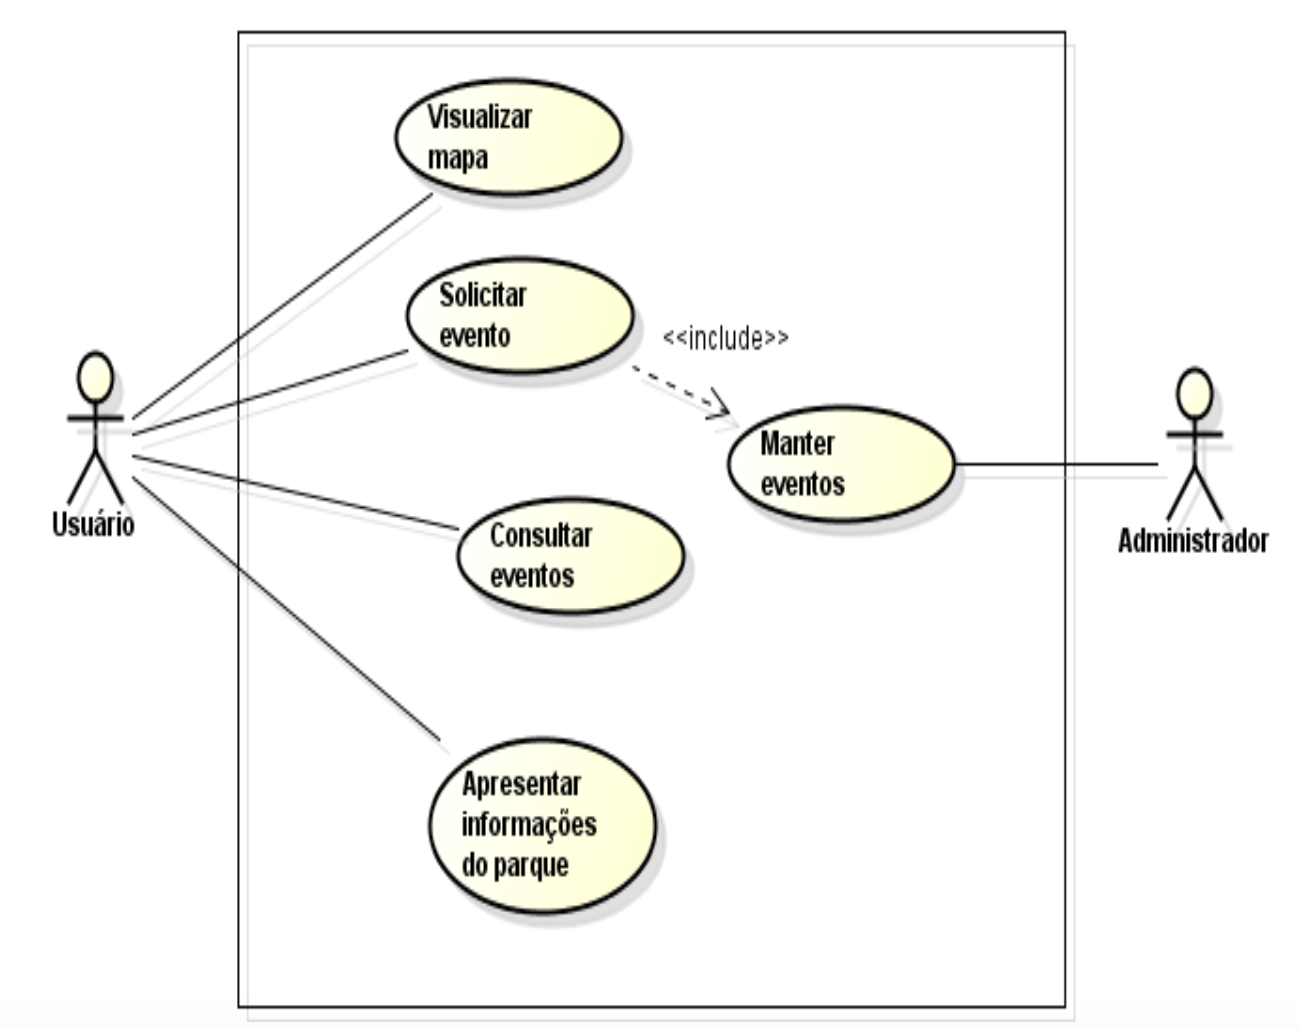
\includegraphics[keepaspectratio=true,scale=0.7]{figuras/DiagramaCasoUso.png}
	\caption{Diagrama de caso de uso do protótipo de software}
\end{figure}

O preço sugerido para o aplicativo é de R\$ 19.000,00. \cite{quantocustaumapp}

\end{anexosenv}

